\section{Pattern: Pattern-Variable Resolution}
\label{section:pv-resolve}

\subsection{Algorithm}

Immediately after parsing the PLTRedex specification, it is unknown whether certain elements of a pattern are built-in patterns, non-terminal symbols or just literals. These elements are represented with \UnresolvedSymbol instances and will have to be resolved in one of the following ways: \BuiltInPatternNoArg, \NonTerminalNoArg, or \LiteralPatternNoArg.

If this transformation is being applied to \texttt{define-language} form, all sub-patterns that resolve to \LiteralPatternNoArg \space need to be stored in set $V$ (initially empty) which is the set of all variables used by the given language. After applying the transformation, \texttt{define-language} $l$ form has to be annotated with $V$ - \MakeAnnotation{$l$}{"ReservedVariables"}{$V$}.

Given \LetDefineLanguage{$l$}, let $\mathit{Nt_{l}}$ be the set of all non-terminal symbols of the language. Given string $\mathit{sym}$, the prefix of $\mathit{sym}$ needs to be extracted. Let $\mathit{prefix_{sym}}$ be a string of characters up to the first occurrence of an underscore character in $\mathit{sym}$. There are several cases to consider.

\begin{itemize}
\item $\mathit{prefix_{sym}}$ does not exist; there are no underscore characters in $\mathit{sym}$. Let $\mathit{prefix_{sym}=sym}$.
\item $\mathit{prefix_{sym}}$ is empty; the first character of $\mathit{sym}$ is underscore. Raise an Exception because PLTRedex doesn't consider such symbols valid.
\item Otherwise, $\mathit{prefix_{sym}}$ is the prefix.
\end{itemize}

The resolution algorithm proceeds in the following manner. The pattern is traversed recursively. When coming across \UnresolvedSymbol \space node, extract $\mathit{prefix_{sym}}$. One of the following cases may happen.

\begin{itemize}
\item Prefix is \texttt{number}, return \BuiltInPattern[Number][$\mathit{sym}$][false].
\item Prefix is \texttt{integer}, return \BuiltInPattern[Integer][$\mathit{sym}$][false].
\item Prefix is \texttt{real}, return \BuiltInPattern[Real][$\mathit{sym}$][false].
\item Prefix is \texttt{natural}, return \BuiltInPattern[Natural][$\mathit{sym}$][false].
\item Prefix is \texttt{string}, return \BuiltInPattern[String][$\mathit{sym}$][false].
\item Prefix is \texttt{boolean}, return \BuiltInPattern[Boolean][$\mathit{sym}$][false].
\item Prefix is \texttt{variable-not-otherwise-mentioned}, \\ return \BuiltInPattern[Variable][$\mathit{sym}$][false]
\item Prefix is \texttt{hole}. Since PLTRedex doesn't allow underscores for \texttt{hole} patterns check if $\mathit{prefix(sym) \neq sym}$ and raise an Exception accordingly. \\ Return \BuiltInPattern[Hole][$\mathit{sym}$][false].
\item $\mathit{prefix_{sym} \in Nt_l}$, return \NonTerminal[$\mathit{prefix_{sym}}$][$\mathit{sym}$][false].
\item Finally, ensure that symbol does not contain underscores. PLTRedex only allows underscores after non-terminal symbols and built-in patterns. Abort compilation process if that is the case. Otherwise, $V=V\cup\{\mathit{sym}\}$ and return \LiteralPattern[Variable][$\mathit{sym}$][false]
\end{itemize}

\subsection{Example}

\begin{figure}[ht]
	\makebox[\textwidth][c] { 
		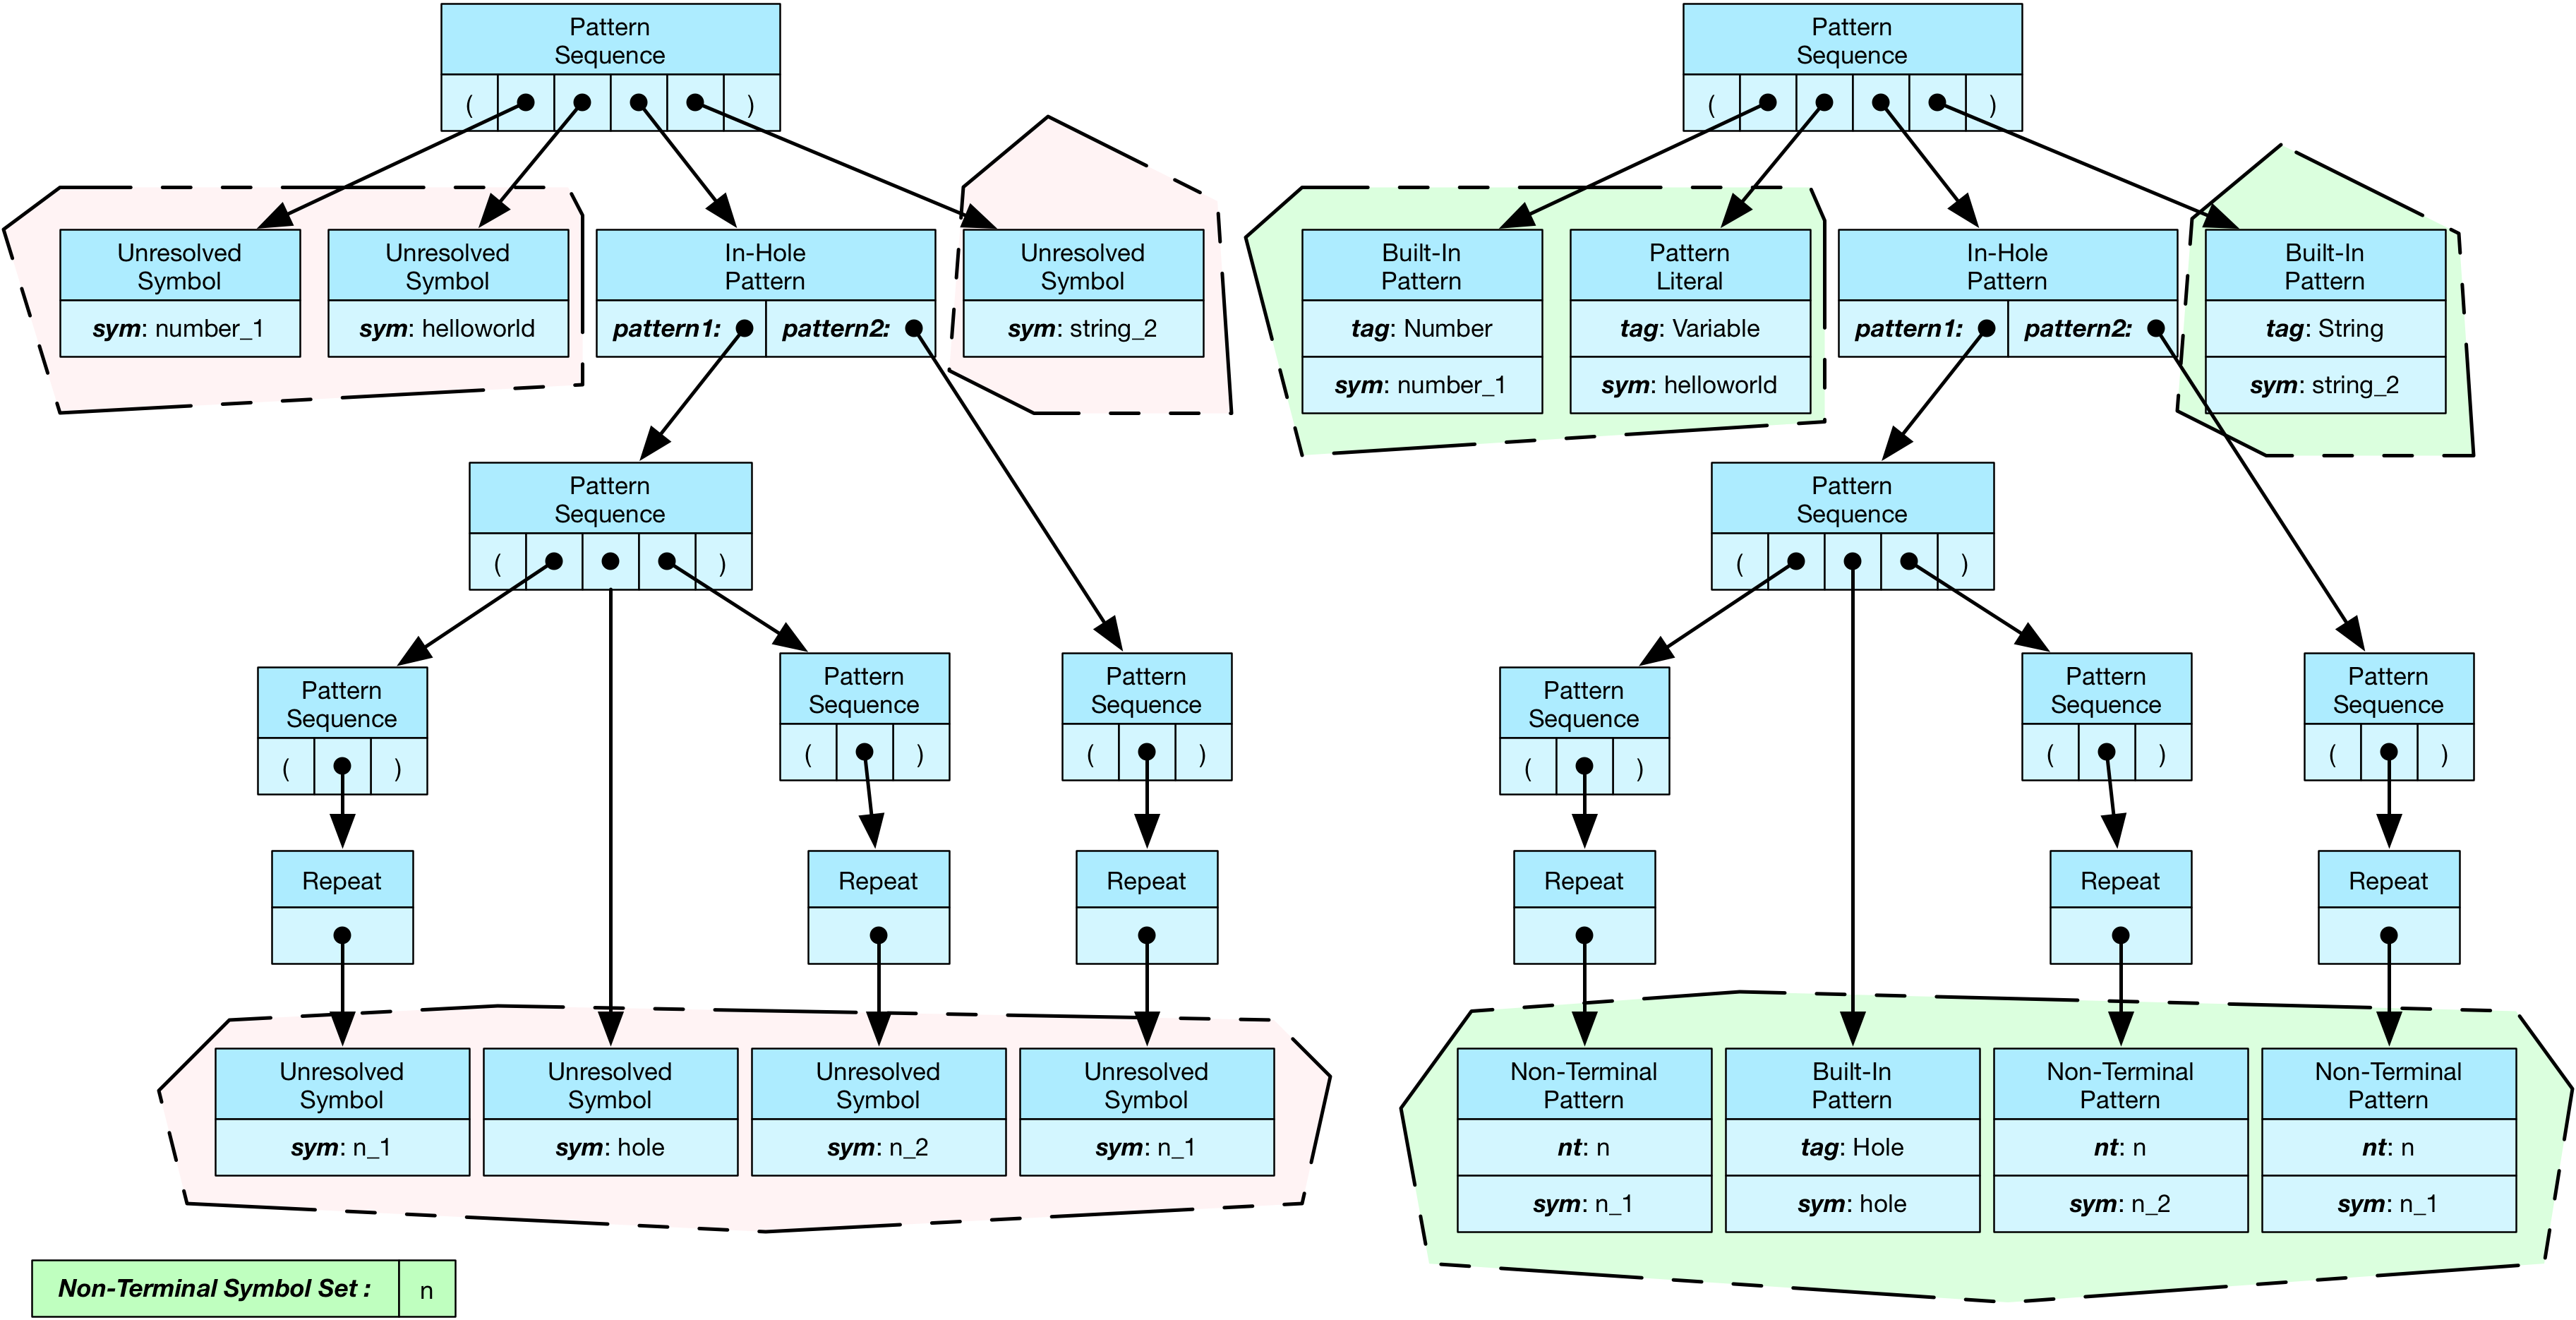
\includegraphics[scale=0.13]{transformation-pattern-resolvesym.png}
	}
\caption{Pattern before and after pattern variable resolution.}
\label{transformation-pattern-resolvesym}
\end{figure}

Figure \ref{transformation-pattern-resolvesym} shows an effect of transformation on pattern \texttt{(number\_1\ helloworld\ (in-hole\ ((n\_1\ ...)\ hole\ (n\_2\ ...))\ (n\_1\ ...))\ string\_2)}. Assume the related \texttt{define-language} has a single non-terminal \texttt{n}. Initially the pattern has six unresolved symbols - \texttt{number\_1}, \texttt{helloworld}, \texttt{n\_1}, \texttt{n\_2}, \texttt{hole} and \texttt{string\_2}. \texttt{number\_1}, \texttt{string\_2}, and \texttt{hole} become \texttt{BuiltInPattern} with appropriate tags,  \texttt{n\_1} and \texttt{n\_2} turn into non-terminals because prefix \texttt{n} is in the set of non-terminal symbols of given \texttt{define-language} and \texttt{helloworld} becomes a \texttt{LiteralPattern} with tag \texttt{Variable}. If this pattern were a part of \texttt{define-language}, \texttt{helloworld} would have been included into set $V$.
